            \subsubsection*{Overfitting with order}
                It's difficult to know how many terms to include in our polynomial, but we run into two problems if our order is \textbf{too high}:

                \begin{itemize}
                    \item It becomes time-consuming to calculate, with little benefit
                    \item We start overfitting more and more.
                \end{itemize}

                The first part makes sense: with more terms, we have to do more multiplications, more additions, etc.\\
                
                \begin{concept}
                    More \vocab{complex models} tend to be more \purp{expensive} to train, and slower to use. This is a trade-off for more \gren{accuracy}. 
                    
                    Usually, there's a point where cost \gren{outweights} benefits. A problem is rarely perfectly solved, even by an excellent model, so you can't just continue until it's "perfect".
                \end{concept}

                But what about the second part? Why do we increase overfitting? 

                With a higher order, our polynomial becomes more complex: it can take on more shapes, which are increasingly complex and perfectly fit to the data.

                This can cause our data to overlook obvious patterns, and instead create a very precise shape that is paying attention to the noise in our model.\\

                \begin{concept}
                    \vocab{High-order polynomials} are very vulnerable to \purp{overfitting}.

                    Because they can take on so many different, \gren{complex} functions, they can very very closely \purp{match} the original data set. 
                    
                    This can cause the model to "learn" noise, and \gren{miss} broader and simpler patterns that actually exist. In may fail to learn something broad and useful, while \purp{memorizing} the dataset with its expressiveness.
                \end{concept}

                Let's see this in action: we'll generate some data based on $2x+1$, while applying some random noise to it. We'll see the optimized linear regression model for each.
                    \note{For ease, we'll exclude regularization: it does help mitigate this problem, but it doesn't totally solve it.}

                Rather than transform the data, we'll transform the separator: this really highlights the overfitting effect.

                \begin{figure}[H]
                    \centering
                    
                    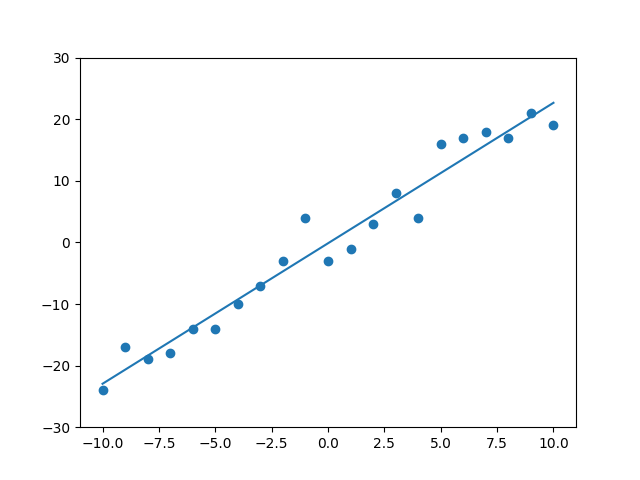
\includegraphics[width=70mm,scale=0.5]{images/feature_images/order_1_soln.png}
                    \caption*{Here's the 1st order solution: in this case, correct for the underlying distribution. It fits our data fine.}
                \end{figure}

                \begin{figure}[H]
                    \centering
                    
                    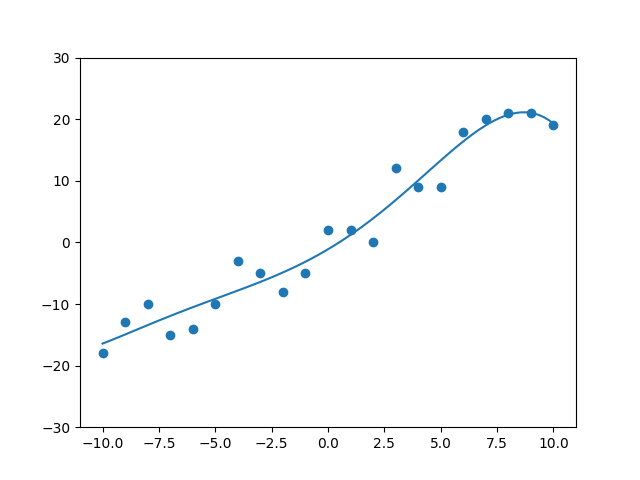
\includegraphics[width=60mm,scale=0.5]{images/feature_images/order_5_soln.png}
                    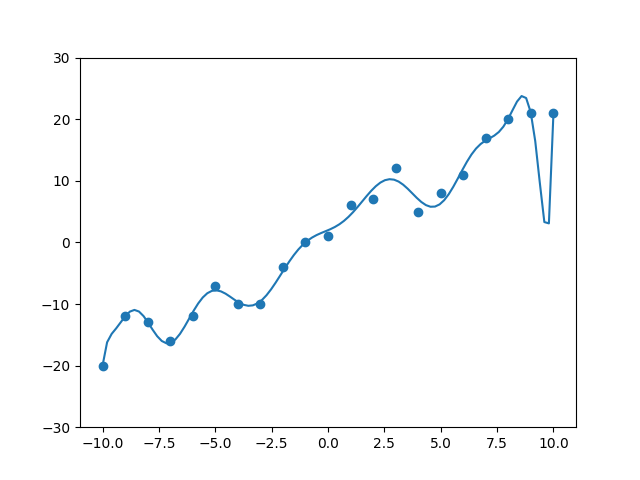
\includegraphics[width=60mm,scale=0.5]{images/feature_images/order_15_soln.png}
                    \caption*{5th and 15th order. The left model looks suspicious, and the right is way overfit. It's very unlikely that we know such an intricate pattern, from so little data.}
                \end{figure}

                 \begin{figure}[H]
                    \centering
                    
                    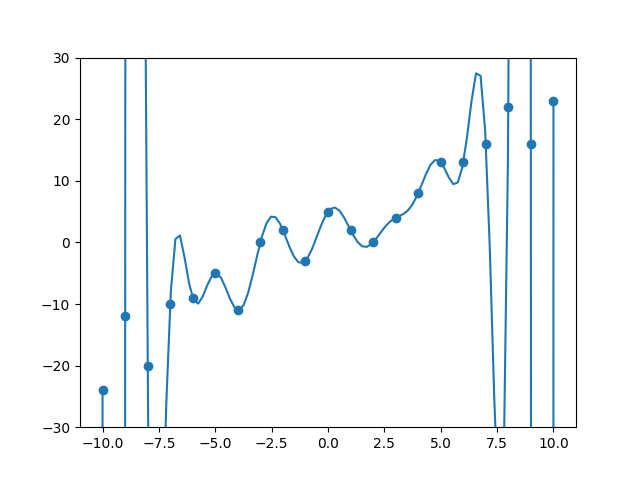
\includegraphics[width=70mm,scale=0.5]{images/feature_images/order_20_soln.png}
                    \caption*{20th order. We have one order for each data point: now, our model is capable of doing regression going through every single data point: as overfit as physically possible, perfectly matching the data.}
                \end{figure}